%
\section{Présentation des simulateurs}
%
%Les simulateurs 
SiCP, SiCF et SiGP sont des programmes permettant l'observation de différents modèles physiques.
\begin{center}
\renewcommand{\arraystretch}{1.1}
\begin{tabular}{ccc}%\begin{center}%\multicolumn{4}{|c|}{}\\%\cline{2-7}\hline
SiCP2  & SiCF & SiGP \\
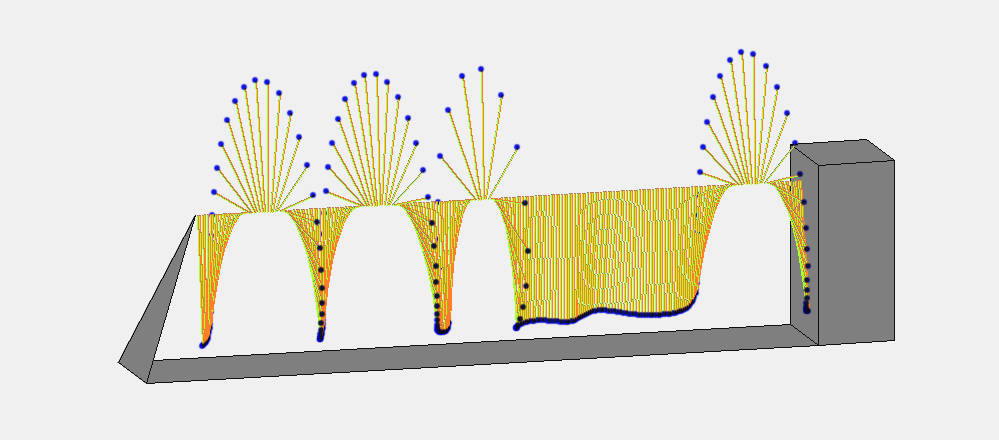
\includegraphics[scale=0.157]{./illustration/SiCP2} & 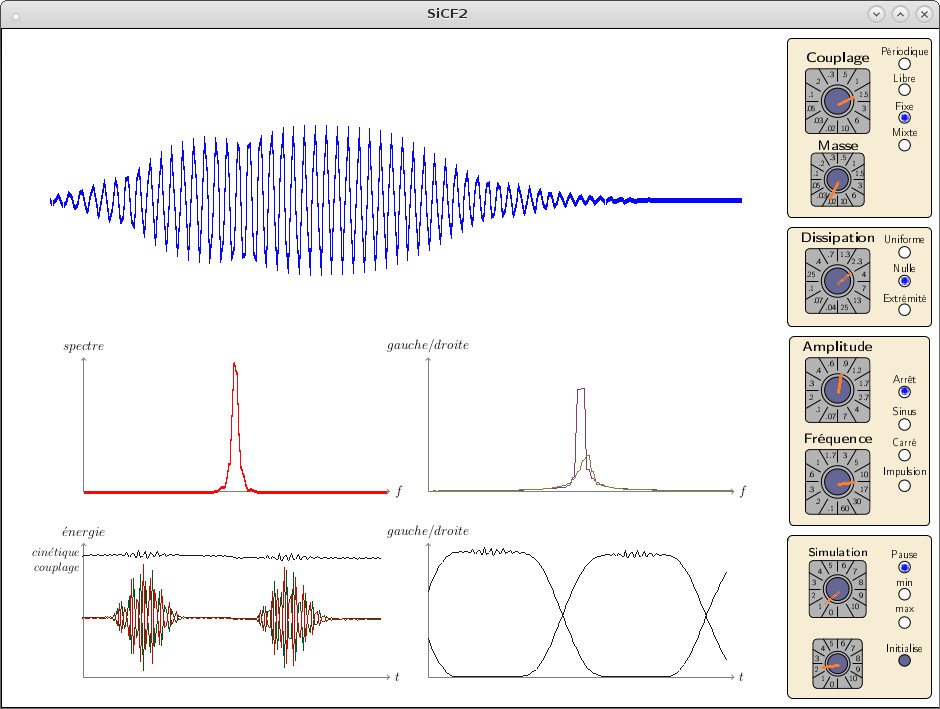
\includegraphics[scale=0.157]{./illustration/SiCF2} & 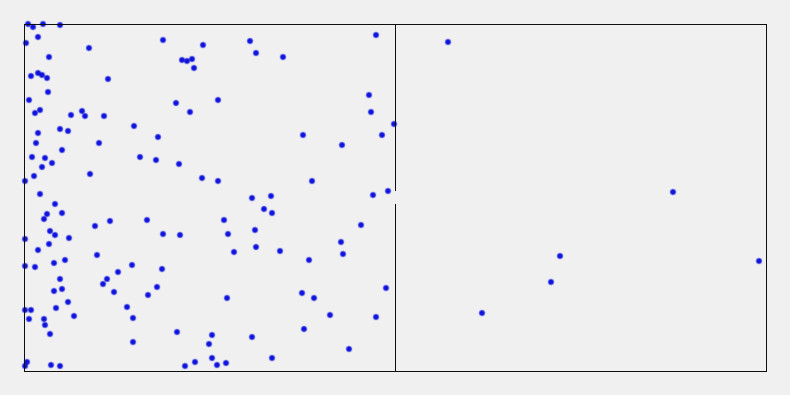
\includegraphics[scale=0.157]{./illustration/SiGP2} \\
Chaîne de pendules  & Corde vibrante & Gaz parfait \\
\end{tabular}
\end{center}
%
Ces programmes offrent une représentation graphique dynamique ainsi qu'une interaction dynamique avec les paramètres physiques.
%Ils permettent également de faire varier l de manière . Les paramètres physiques 
%
%\subsection{SiCF et SiCP, simulateurs d'oscillateurs couplés}
%SiCF et SiCP sont des simulateurs d'oscillateurs couplés à une dimension.
\subsection{SiCP2, chaîne de pendules couplés}
%
SiCP est un simulateur de chaîne de pendule. Un moteur sinusoïdale, carré, ou impulsionnel permet de créer une excitation de l'extrémité de la chaîne. Les conditions aux limites peuvent être périodiques, libres ou fixes. La dissipation peut être uniforme ou simuler une extrémité absorbante.
%
\begin{center}
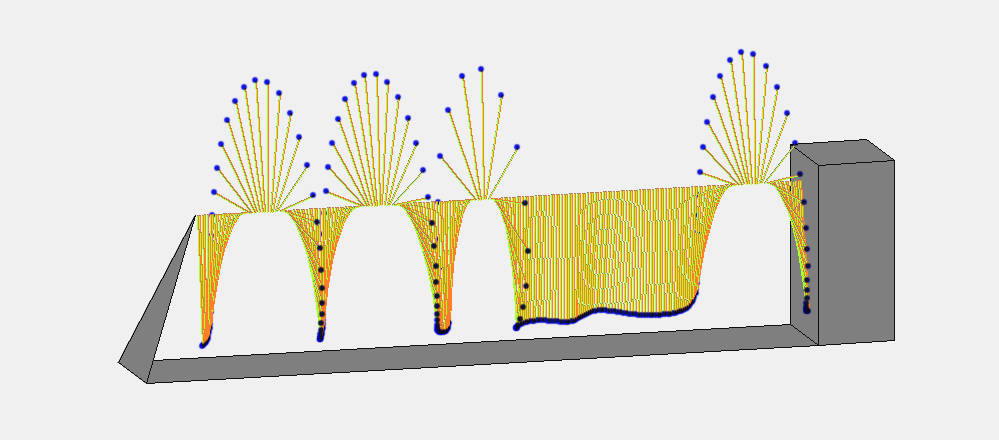
\includegraphics[scale=0.41]{./illustration/SiCP2}
\end{center}
%
Le programme simule l'équation de sine-gordon. Le contrôle du courant josephson permet d'observer la dynamique des solitons.
%\item Graphisme en 3 dimensions, déplacement du point du vue.
%Le programme possède une interface permettant le contrôle de la simulation à l'aide de la souris.
\subsection{SiCF, corde vibrante et transformée de fourier}
%
SiCF est un simulateur de corde vibrante permettant la visualisation du spectre en fréquence spatiale de la corde. Un moteur sinusoïdale, carré, ou impulsionnel permet de créer une excitation de l'extrémité de la corde. Les conditions aux limites peuvent être périodiques, libres ou fixes. La dissipation peut être uniforme ou simuler une extrémité absorbante.

Une dissymétrie de la corde permet d'observer les phénomènes de réflexion et de transmission.

\begin{center}
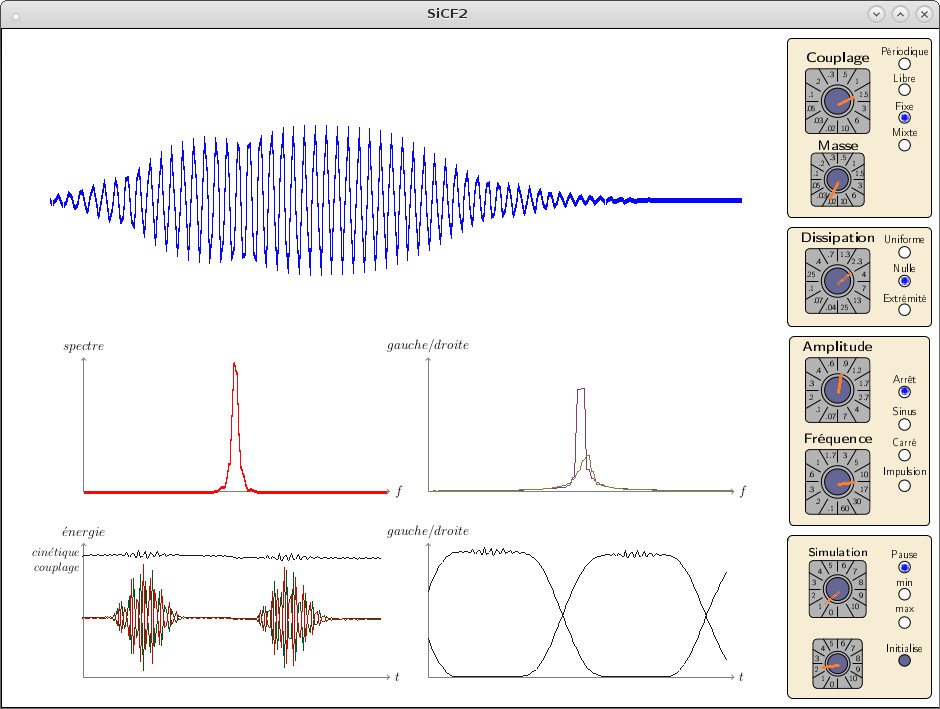
\includegraphics[scale=0.51]{./illustration/SiCF2}
\end{center}
%
Le programme simule l'équation de la corde vibrante et calcule la transformée de fourier des moitiés droite et gauche de la corde.

%La fenêtre graphique montre une Représentation du spectre.
%\item Enregistrement et rechargement des situations.
%\item Conditions initiales préenregistrées.
%
\subsection{SiGP, thermodynamique statistique}
%
Le simulateur de gaz parfait SiGP permet de visualiser une interprétation statistique de la détente de Joule, du démon de Maxwell ainsi que du contact avec un ou deux thermostats.
%
\begin{center}
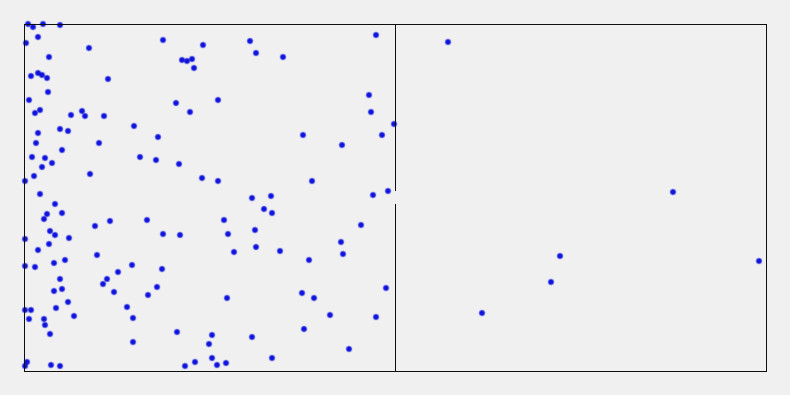
\includegraphics[scale=0.41]{./illustration/SiGP2}
\end{center}
%
Le programme simule des collisions élastiques de particules entre elles et avec les parois ainsi que l'interaction avec un thermostat.
%
La paroi centrale permet d'observer une détente de joule ou l'action d'un démon de Maxwel.
%
%%%%%%%%%%%%%%%%%%%%%%%%%%%%%%%%%%%%%%%%%%%%%%%%%%%%%%%%%%%%%%%%%%%%%%%%%%%%%%%%%%%%%%%%%%%%%
